% CREATED BY DAVID FRISK, 2018
\chapter{Introducción}\label{introduccion}

Este Trabajo de Fin de Máster aborda el aprendizaje por refuerzo para el control visual de un robot. Se encuadra en la intersección de tres áreas de interés creciente: la visión artificial, el aprendizaje automático y la robótica.\\

En este capítulo se introduce el tema general del proyecto, aprendizaje por refuerzo para control visual de un robot y la motivación que lleva a la resolución del problema y se fijan los objetivos concretos a abordar.

%%%%%%%%%%%%%%%%%%%%%%%%%%%%%%%%%%%%%%%%%%%%%%%%%%%%%%%%%%%%%%%%%%%%%%%%%%%%%%%%%%%%%%%%%%%%%%%%%%%%%%%%%%%%%%%%
\section{Motivación y contexto}\label{motivacion}


En la última década se está viviendo una explosión de los campos de la inteligencia artificial y la robótica en muchos de los ámbitos que nos rodean: social, político, médico, tecnológico, etc. Muchos de estos cambios promovidos por la inteligencia artificial que vive constantes renovaciones y revisiones de sí misma donde los repositorios que contienen el código con meses de antigüedad parezcan piezas de museo haciendo que el tiempo, en vez de años, parezcan siglos.\\

Por ejemplo, en el campo del procesamiento natural del lenguaje parece que fue el <<siglo pasado>> cuando OpenAI lanzó su popular modelo de generación de texto en su versión 2; (\textit{Generative Pre-trained Transformer} o GPT-2) que tanto impresionó al mundo con los textos y conversaciones que tenían dos máquinas dándoles únicamente una pequeña semilla. Esto ocurrió a principios del 2019. Este modelo ha pasado a un segundo plano por culpa de su hermano mayor, el generador de texto en su versión 3 (GPT-3) que contiene una cantidad mayor de parámetros y es capaz de mantener conversaciones similares a las de un humano sin aparente esfuerzo.\\

El incremento del uso de la \textit{inteligencia artificial} en cada vez más ámbitos viene también impulsado por el aumento de la capacidad de cómputo de los procesadores, mayor número de núcleos para el procesamiento, capaces de paralelizar más procesos, aceleración por hardware, aumento del número de librerías que facilitan el uso de esta tecnología (TensorFlow, Pytorch, etc) así como la reducción del coste de los componentes y sensores y la accesibilidad para realizar programas complejos con elementos casi domésticos.\\

Esta explosión en el campo de la inteligencia artificial viene cimentada sobre una base que comenzó a construirse desde la creación de la considerada primera neurona artificial, el perceptrón (1958). Desde su nacimiento, el interés por el aprendizaje automático ha ido en constante crecimiento con la creación de diferentes algoritmos de aprendizaje automático \textit{supervisado} como los clasificadores, árboles de decisión, máquinas de vector soporte (\textit{Support Vector Machine}, SVM), \textit{no supervisado} como: agrupación (\textit{clustering}), o la rama más psicológica del \textit{aprendizaje por refuerzo} con algoritmos como QLearn, SARSA, etc.\\

En el año 2012 se produce un nuevo crecimiento en este campo con la solución presentada en el reto del reconocimiento visual a gran escala con el conjunto de datos\footnote{\url{http://image-net.org/challenges/LSVRC/}} <<Image Net>>\footnote{\url{http://www.image-net.org/}}, el \textit{aprendizaje profundo} o \textit{Deep Learning}. Con esta solución, muchos de los algoritmos conocidos evolucionan a su versión con la nueva arquitectura donde los resultados mejorarían drásticamente debido a la capacidad de generalización que se consigue, donde es la propia red neuronal la que aprende las características de los datos que van pasando por ella.\\

En al ámbito de la \textit{visión por computador}, los avances han sido igualmente sorprendentes para un gran abanico de tareas como son: la segmentación (figura \ref{fig:intro_segmentacion}), detección (figura \ref{fig:intro_deteccion}), reconocimiento (figura \ref{fig:intro_reconocimiento}), restauración (figura \ref{fig:intro_restauracion}), pose corporal, gestos, etc. En todos ellos, el estado actual está muy avanzado debido a las constantes revisiones de los trabajos y el incremento en capacidad de cómputo así como el interés que despierta el campo de la visión en muchos sectores como puede ser: industrial, civil, social, etc.\\

\begin{figure}[ht!]
  \begin{center}
    \subfloat[Segmentación.]{\label{fig:intro_segmentacion}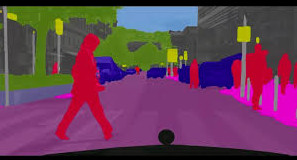
\includegraphics[width=.45\linewidth]{figures/chapter_1/segmentation.jpg}}
    \hspace{0.1cm}
    \subfloat[Detección.]{\label{fig:intro_deteccion}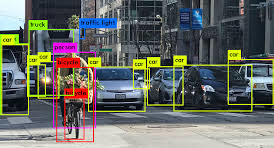
\includegraphics[width=.45\linewidth]{figures/chapter_1/detection.jpg}}
    \hspace{0.1cm}
    \subfloat[Reconocimiento facial.]{\label{fig:intro_reconocimiento}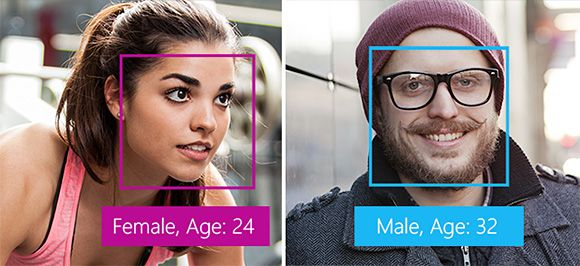
\includegraphics[width=.45\linewidth]{figures/chapter_1/face.detection.jpg}}
    \hspace{0.1cm}
    \subfloat[Restauración.]{\label{fig:intro_restauracion}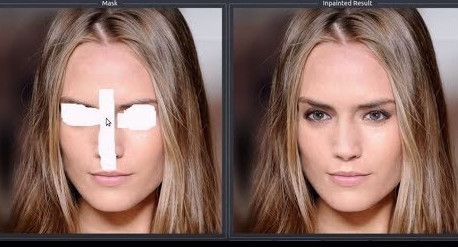
\includegraphics[width=.45\linewidth]{figures/chapter_1/inpainting.jpg}}
  \end{center}
  \centering
  \captionsetup{justification=centering,margin=2cm}
  \caption{Ejemplos de soluciones de visión artificial.}
  \label{fig:robots-gym-gazebo}
\end{figure}


Por otro lado, la combinación de la robótica y la inteligencia artificial, genera soluciones que podemos ver en muchos campos como el médico (robot de cirujía DaVinci\footnote{\url{http://www.abexsl.es/es/robot-da-vinci/que-es}}), doméstico (aspiradores Roomba\footnote{\url{https://www.irobot.es/}}), logístico (movimiento de mercancía en almacenes, como Amazon\footnote{\url{https://www.wired.com/story/amazon-warehouse-robots/}}), automovilístico (conducción semi-autónoma de Tesla Motors, Inc\footnote{\url{https://www.tesla.com/es_es}}), dotando de distintos tipos de sensores y en muchos de ellos con uno en común, el sensor de imagen o cámara. Y es en este punto donde se ha potenciado el uso de la inteligencia artificial y su capacidad para extraer \textit{información valiosa} (características) de imágenes con precisión en función de la aplicación, habiéndose entrenado previamente para solucionar esa tarea en concreto. La reducción del coste de este componente facilita además su integración en todo tipo de dispositivos por lo que es más accesible integrar soluciones basadas en este campo de la inteligencia artificial, la \textit{visión por computador}.\\

\begin{figure}[ht!]
  \begin{center}
    \subfloat[Robot DaVinci.]{\label{fig:davinci-robot}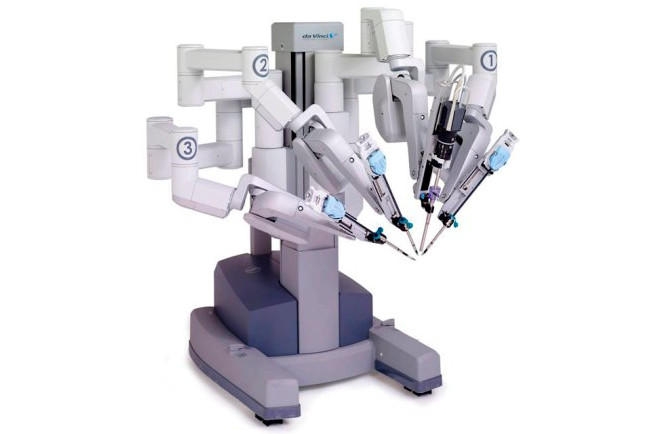
\includegraphics[width=.45\linewidth]{figures/chapter_1/davinci-robot.jpg}}
    \hspace{0.1cm}
    \subfloat[Robots Aspiradores.]{\label{fig:aspiradores-robot}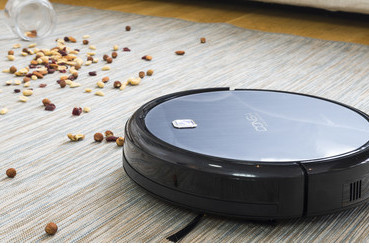
\includegraphics[width=.45\linewidth]{figures/chapter_1/aspirador-robot.jpg}}
    \hspace{0.1cm}
    \subfloat[Robots de almacén.]{\label{fig:amazon-robot}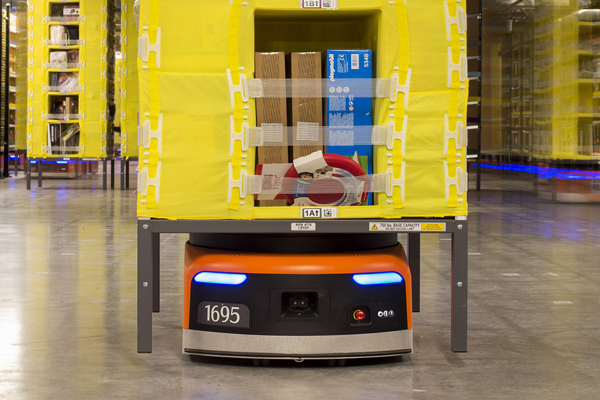
\includegraphics[width=.45\linewidth]{figures/chapter_1/amazon-robot.png}}
    \hspace{0.1cm}
    \subfloat[Coches semi-autónomos.]{\label{fig:tesla-robot}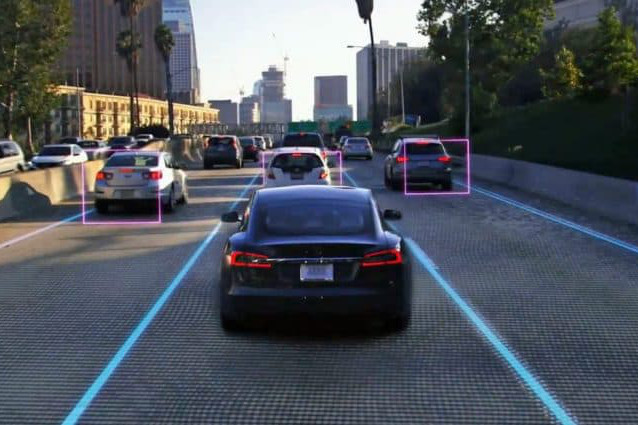
\includegraphics[width=.45\linewidth]{figures/chapter_1/tesla-robot.jpg}}
  \end{center}
  \centering
  \captionsetup{justification=centering,margin=2cm}
  \caption{Aplicaciones robóticas.}
  \label{fig:robots-gym-gazebo}
\end{figure}


La compañía Nvidia\footnote{\url{https://www.nvidia.com/es-es/}}, la mayor empresa en la creación de tarjetas aceleradoras hardware, cuenta también con soluciones que combinan ambos campos. Cuenta con un departamento de enseñanza robótica a través de su robot Jetbot\footnote{\url{https://www.nvidia.com/es-es/autonomous-machines/embedded-systems/jetbot-ai-robot-kit/}} (figura \ref{fig:jetbot}), que incorpora una tarjeta gráfica para la aceleración de los cálculos en los algoritmos de inteligencia artificial en la propia placa (Jetson Nano, Xavier, TX, etc) así como una cámara como sensor principal. Esto permite construir vehículos gobernados por algoritmos inteligentes a un coste cada vez más ajustado para resolver problemas como seguir una carretera o leer señales de tráfico para detener el robot gracias al sensor visual que le permite <<ver>> y <<entender>> los elementos que le rodean.

\begin{figure}[!ht]
    \centering 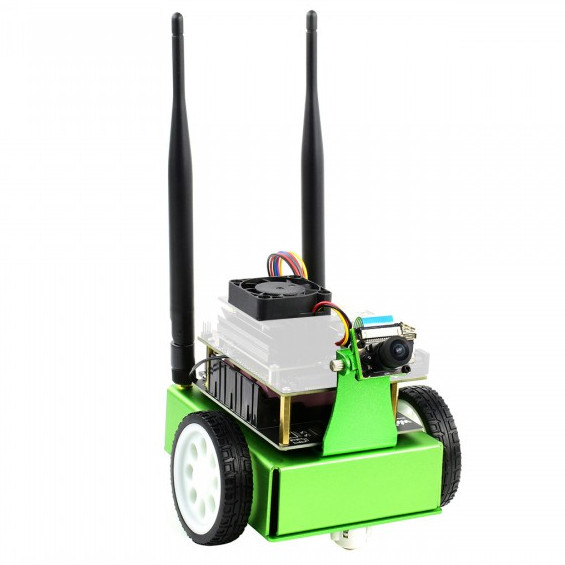
\includegraphics[width=0.4\columnwidth]{figures/chapter_1/jetbot.jpg}
    \caption{Robot para robótica educativa de Nvidia, Jetbot.}\label{fig:jetbot}
\end{figure}

A nivel industrial, el crecimiento de robots ha ido en aumento desde el 2018~\cite{robotica_industrial} (un 6\% de incremento) y se pronostica que ese incremento vaya ampliándose año tras año. Además de la apuesta de países como China, Japón, República de Corea, Estados Unidos y Alemania por la robótica, el sector automovilístico está siendo el que más demanda la robótica a nivel mundial, promovido por la actualización de las cadenas de montaje así como el creciente impulso que se está destinando a los nuevos vehículos eléctricos. En la figura \ref{fig:crecimiento_robotica_industrial} puede verse un gráfico con la tendencia creciente en la última década en el sector.

\begin{figure}[!ht]
    \centering 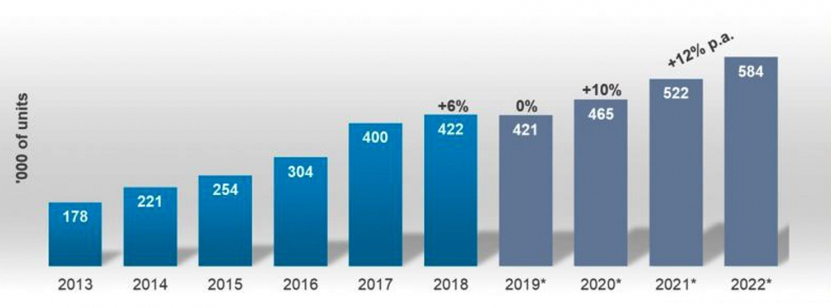
\includegraphics[width=0.9\columnwidth]{figures/chapter_1/robotica_grafico.jpeg}
    \caption{Previsión de crecimiento de la robótica industrial desde el 2013. Fuente: World Robotics 2019.}\label{fig:crecimiento_robotica_industrial}
\end{figure}

La industria automovilística está revolucionando el mercado incorporando en los coches mecanismos de conducción, por el momento, semi-autónoma que gestionan el comportamiento y ayudan en la conducción y proporcionan un componente más de seguridad. Esta revolución dentro del sector ha sido protagonizado los últimos años por la empresa Tesla Motors, Inc, que combina todo lo mencionado en este punto: varias cámaras para recoger información, hardware que procesa la información del sensor, software que procesa, gestiona y actúa en base a unas decisiones tomadas por algoritmos de inteligencia artificial que procesan estas imágenes de entrada hasta en condiciones extremas.\\

En la figura \ref{fig:tesla-view} puede verse un ejemplo muy simplificado de cómo las cámaras del vehículo puede detectar otros a su alrededor así como segmentar el carril por el que circula y sus aledaños.

\begin{figure}[!ht]
    \centering 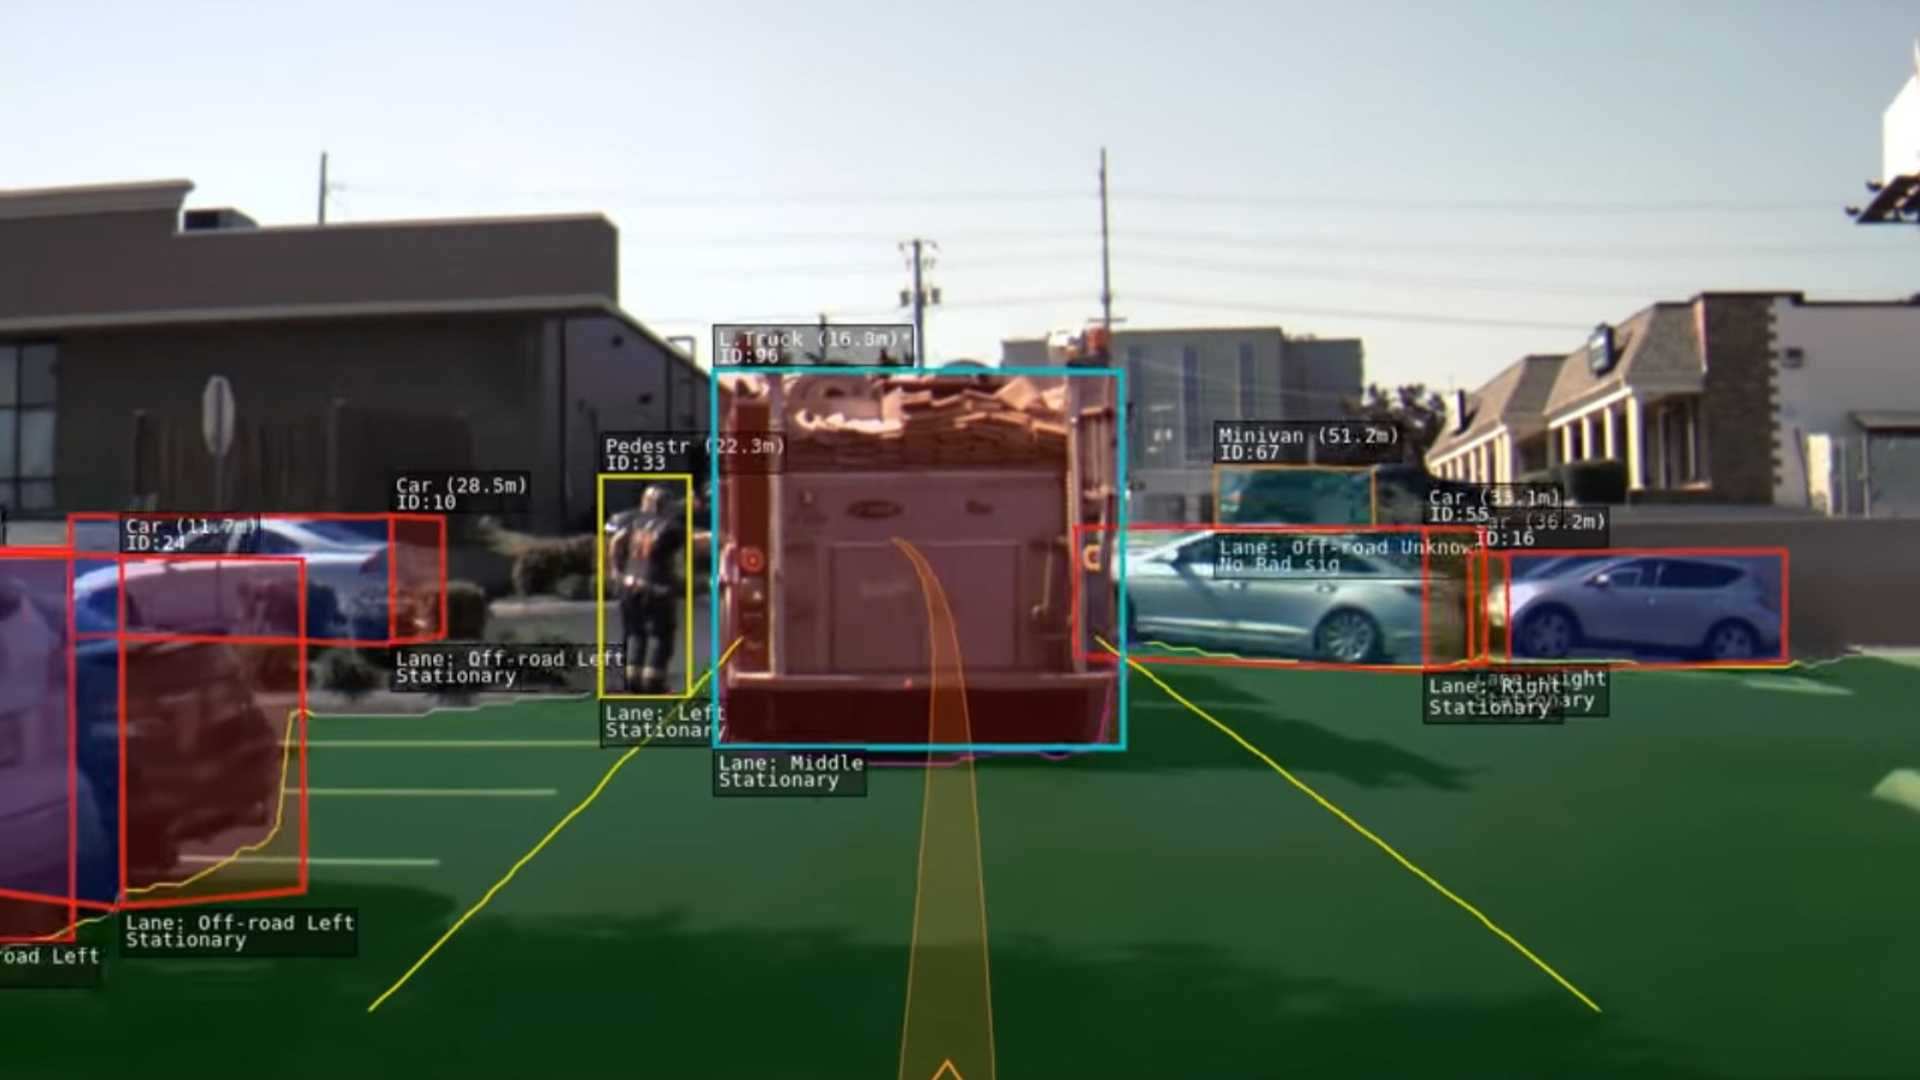
\includegraphics[width=0.7\columnwidth]{./figures/chapter_1/tesla-view.jpg}
    \caption{Visión de un vehículo Tesla a través de la cámara.}\label{fig:tesla-view}
\end{figure}

Esta detección puede extenderse a la de peatones, bicicletas, distancia de seguridad con vehículos posteriores, navegación automática, cambio de carril, etc.\\

Para conseguir este hito de la historia contemporánea ha hecho falta entrenar algoritmos de inteligencia artificial que sean capaces de tomar las mejores decisiones en cada una de las situaciones a las que se enfrentan. Para ello es necesario alimentar al sistema con imágenes de todo tipo de iluminación y visibilidad: lluvia, nieve, niebla, soleado, nublado, etc.\\

Estos procesos de entrenamiento pueden llevarse a cabo de varias maneras como puede ser: clasificar una imagen tomada de lluvia, segmentar el carril y tomar una decisión o, el tema de este trabajo, enseñar a vehículos a resolver el problema de seguir un carril o una línea utilizando otro tipo de aprendizaje automático: \textit{el aprendizaje por refuerzo}.


%%%%%%%%%%%%%%%%%%%%%%%%%%%%%%%%%%%%%%%%%%%%%%%%%%%%%%%%%%%%%%%%%%%%%%%%%%%%%%%%%%%%%%%%%%%%%%%%%%%%%%%%%%%%%%%%
\section{Objetivos y requisitos}\label{objetivos}

El objetivo principal del proyecto es entrenar un vehículo en un simulador para seguir la línea dibujada en el asfalto utilizando aprendizaje por refuerzo. El resultado de estos entrenamientos será un vehículo capaz de recorrer un circuito de manera autónoma y comprobar si es capaz de solucionar circuitos para los que no ha sido entrenado. Estos objetivos se dividen en:\\

\begin{enumerate}
    \item Programar un entorno de aprendizaje por refuerzo con visión y robots.\\
    \item Entrenar un controlador visual para conducción autónoma siguiendo una línea.\\
    \item Validación experimental y análisis de las posibilidades del aprendizaje por refuerzo.\\
\end{enumerate}

Todos los puntos mencionados son resueltos usando siempre la cámara como sensor de entrada de información que, mediante un procesamiento de cada imagen, se ofrecerá como respuesta a los motores en forma de movimiento.\\

Para la elaboración del trabajo del fin de máster se listan los siguientes requisitos:\\

\begin{itemize}
    \item Uso del sistema operativo robótico (\textit{Robot Operating System}, ROS) como interfaz para la comunicación con el robot.
    \item Uso del simulador Gazebo para realizar las pruebas en diferentes circuitos.
    \item Emplear aprendizaje por refuerzo como herramienta de entrenamiento del robot a través del entorno Gym-Gazebo.
\end{itemize}



%%%%%%%%%%%%%%%%%%%%%%%%%%%%%%%%%%%%%%%%%%%%%%%%%%%%%%%%%%%%%%%%%%%%%%%%%%%%%%%%%%%%%%%%%%%%%%%%%%%%%%%%%%%%%%%%
\section{Metodología}

Para este trabajo de fin de máster se ha empleado el método de desarrollo en espiral, muy usado en ingenierı́a de software y que permite establecer pequeños objetivos para cada una de la iteraciones, formado por un conjunto de actividades. Estas actividades consisten en establecer unos objetivos, planificados previamente en función de los cumplidos en la semana anterior.\\

Estructurados por prioridad, se estudia su diseño y se programa una solución. Una vez resuelto se procede a pruebas de los componentes y se evalúan los resultados y objetivos marcados de cara a proponer unos nuevos, comenzando una nueva iteración en el bucle. En la figura \ref{fig:metodo_espiral}, se muestra un diagrama con la estructura de la metodologı́a seguida durante el desarrollo del proyecto.

\begin{figure}[!ht]
    \centering 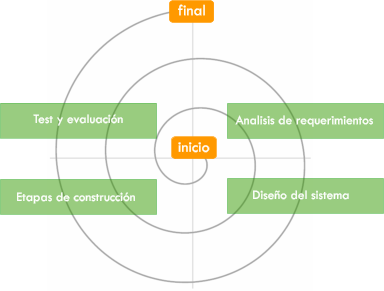
\includegraphics[width=0.6\columnwidth]{figures/chapter_1/metodo_espiral.png}
    \caption{
        \label{fig:metodo_espiral}
            Método en espiral
    }
\end{figure}

Desde el comienzo de este trabajo, se han planificado reuniones semanales con los tutores en el que se analizaba el progreso y objetivos y se marcaban los de la siguiente semana siguiendo el esquema en espiral.\\

El código desarrollado se almacena en un repositorio público de GitHub (\url{https://github.com/RoboticsLabURJC/2019-tfm-ignacio-arranz}), perteneciente a RoboticsLabURJC\footnote{\url{https://github.com/RoboticsLabURJC}} de la Universidad Rey Juan Carlos donde se guarda un registro con todos los cambios. Además, en el mismo repositorio se crea un \textit{blog}\footnote{\url{https://roboticslaburjc.github.io/2019-tfm-ignacio-arranz/}} sobre el proyecto en el que se escriben los avances semanales/mensuales desde el comienzo del desarrollo hasta la solución final.


%%%%%%%%%%%%%%%%%%%%%%%%%%%%%%%%%%%%%%%%%%%%%%%%%%%%%%%%%%%%%%%%%%%%%%%%%%%%%%%%%%%%%%%%%%%%%%%%%%%%%%%%%%%%%%%%
\section{Estructura del documento.}\label{estructura_documento}

La estructura del trabajo presentado está compuesta por los siguientes capítulos:\\

\begin{itemize}
    \item \textbf{Capítulo 1}: Se presenta una introducción al proyecto así como la motivación que ha llevado a resolver la tarea y los objetivos que se pretenden alcanzar.\\
    \item \textbf{Capítulo 2}: En el estado del arte se presenta el posicionamiento del proyecto dentro del marco de trabajos similares.\\
    \item \textbf{Capítulo 3}: Describe cada una de las herramientas empleadas en el proyecto.\\
    \item \textbf{Capítulo 4}: Programación del código de aprendizaje por refuerzo para el control visual.\\
    \item \textbf{Capítulo 5}: Estudios y resultados experimentales.\\
    \item \textbf{Capítulo 6}: Se extraen conclusiones de todo lo desarrollado anteriormente y la línea de trabajos por la que se pretende continuar con el proyecto.\\
\end{itemize}

\noindent
Los anexos a este proyecto se utilizan para proporcionar la información de tablas, imágenes o fragmentos de código que complementen los resultados.
